\documentclass[tikz,border=5pt]{standalone}
\usepackage{tikz}
\usetikzlibrary{shapes.geometric,arrows.meta,positioning,fit,backgrounds,shadows}

\begin{document}
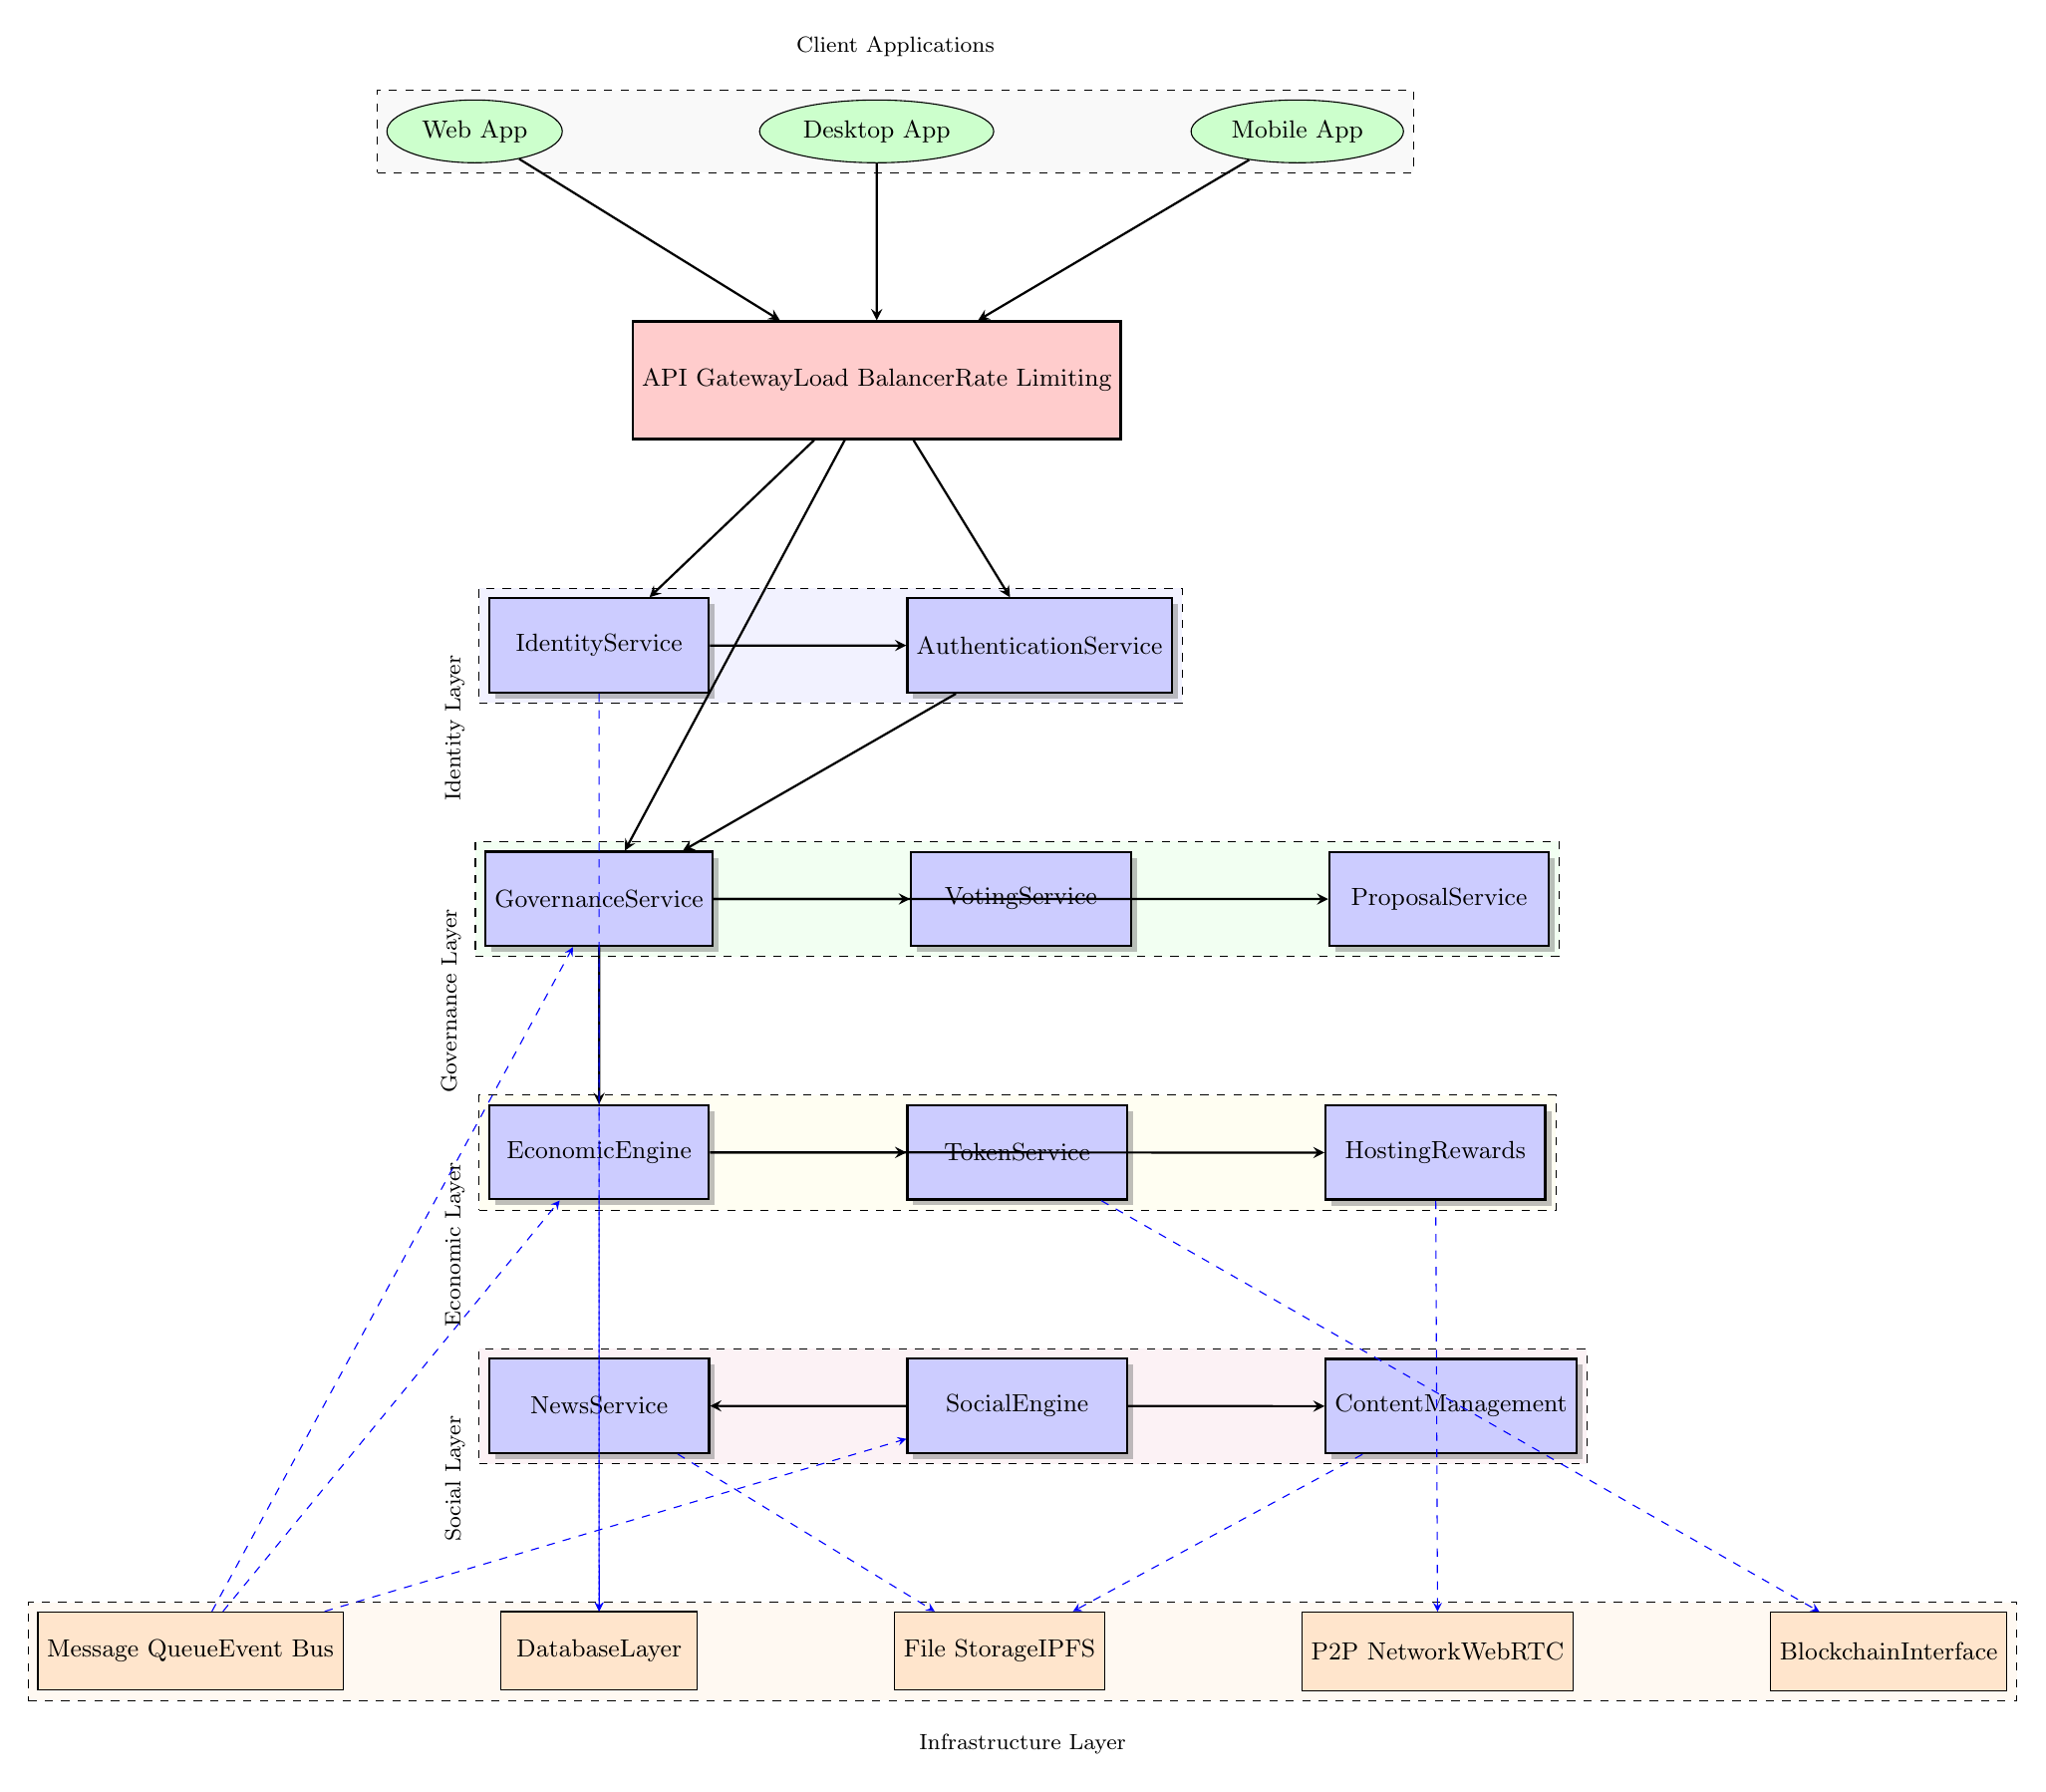
\begin{tikzpicture}[scale=1.5,
    node distance=2.5cm,
    every node/.style={font=\small},
    service/.style={rectangle,draw,minimum width=2.8cm,minimum height=1.2cm,fill=blue!20,thick,drop shadow},
    gateway/.style={rectangle,draw,minimum width=3cm,minimum height=1.5cm,fill=red!20,thick},
    infra/.style={rectangle,draw,minimum width=2.5cm,minimum height=1cm,fill=orange!20},
    client/.style={ellipse,draw,minimum width=2cm,minimum height=0.8cm,fill=green!20},
    arrow/.style={->,>=stealth,thick},
    data/.style={->,>=stealth,dashed,blue}
]

% Client Applications
\node[client] (web) {Web App};
\node[client,right=of web] (desktop) {Desktop App};
\node[client,right=of desktop] (mobile) {Mobile App};

% API Gateway
\node[gateway,below=2cm of desktop] (gateway) {API Gateway\\Load Balancer\\Rate Limiting};

% Core Services - Identity Layer
\node[service,below left=2cm and -1cm of gateway] (identity) {Identity\\Service};
\node[service,right=of identity] (auth) {Authentication\\Service};

% Core Services - Governance Layer
\node[service,below=2cm of identity] (governance) {Governance\\Service};
\node[service,right=of governance] (voting) {Voting\\Service};
\node[service,right=of voting] (proposal) {Proposal\\Service};

% Core Services - Economic Layer  
\node[service,below=2cm of governance] (economy) {Economic\\Engine};
\node[service,right=of economy] (token) {Token\\Service};
\node[service,right=of token] (hosting) {Hosting\\Rewards};

% Core Services - Social Layer
\node[service,below=2cm of economy] (news) {News\\Service};
\node[service,right=of news] (social) {Social\\Engine};
\node[service,right=of social] (content) {Content\\Management};

% Infrastructure Services
\node[infra,below=2cm of news] (database) {Database\\Layer};
\node[infra,right=of database] (storage) {File Storage\\IPFS};
\node[infra,right=of storage] (p2p) {P2P Network\\WebRTC};
\node[infra,right=of p2p] (blockchain) {Blockchain\\Interface};

% Message Queue
\node[infra,left=2cm of database] (queue) {Message Queue\\Event Bus};

% Background groupings
\begin{scope}[on background layer]
\node[fill=gray!5,draw,dashed,fit=(web)(desktop)(mobile)] (clientgroup) {};
\node[fill=blue!5,draw,dashed,fit=(identity)(auth)] (identitygroup) {};
\node[fill=green!5,draw,dashed,fit=(governance)(voting)(proposal)] (govgroup) {};
\node[fill=yellow!5,draw,dashed,fit=(economy)(token)(hosting)] (econgroup) {};
\node[fill=purple!5,draw,dashed,fit=(news)(social)(content)] (socialgroup) {};
\node[fill=orange!5,draw,dashed,fit=(database)(storage)(p2p)(blockchain)(queue)] (infragroup) {};
\end{scope}

% Client to Gateway connections
\draw[arrow] (web) -- (gateway);
\draw[arrow] (desktop) -- (gateway);
\draw[arrow] (mobile) -- (gateway);

% Gateway to Services
\draw[arrow] (gateway) -- (identity);
\draw[arrow] (gateway) -- (auth);
\draw[arrow] (gateway) -- (governance);

% Inter-service connections
\draw[arrow] (identity) -- (auth);
\draw[arrow] (auth) -- (governance);
\draw[arrow] (governance) -- (voting);
\draw[arrow] (governance) -- (proposal);
\draw[arrow] (governance) -- (economy);
\draw[arrow] (economy) -- (token);
\draw[arrow] (economy) -- (hosting);
\draw[arrow] (social) -- (news);
\draw[arrow] (social) -- (content);

% Service to Infrastructure connections
\draw[data] (identity) -- (database);
\draw[data] (governance) -- (database);
\draw[data] (economy) -- (database);
\draw[data] (news) -- (storage);
\draw[data] (content) -- (storage);
\draw[data] (hosting) -- (p2p);
\draw[data] (token) -- (blockchain);

% Message Queue connections
\draw[data] (queue) -- (governance);
\draw[data] (queue) -- (economy);
\draw[data] (queue) -- (social);

% Labels
\node[above=0.3cm of clientgroup,font=\footnotesize] {Client Applications};
\node[left=0.3cm of identitygroup,font=\footnotesize,rotate=90] {Identity Layer};
\node[left=0.3cm of govgroup,font=\footnotesize,rotate=90] {Governance Layer};
\node[left=0.3cm of econgroup,font=\footnotesize,rotate=90] {Economic Layer};
\node[left=0.3cm of socialgroup,font=\footnotesize,rotate=90] {Social Layer};
\node[below=0.3cm of infragroup,font=\footnotesize] {Infrastructure Layer};

\end{tikzpicture}
\end{document}
